\section{Introduzione}
Il pendolo invertito su rotaia è un sistema facile da modellare
ma presenta alcune caratterische che rendono interessante studiarne la controllabilità.
Il sistema è mostrato in figura \ref{fig:pic} e consiste in un pendolo rigido, libero di ruotare e vincolato a muoversi lungo una rotaia rettilinea tramite un carrello. L'unico modo in cui i sistema può interagire con l'esterno è tramite una forza applicata sul carrello lungo la direzione della rotaia. Quando il pendolo è fermo ed è diretto verso l'alto, si trova in un punti di equilibrio instabile e ogni minima perturbazione tenderà a farlo ricadere verso il basso. L'obiettivo che mi pongo è duplice:

\begin{enumerate}
    \item Stabilizzare il pendolo attorno al punto di equilibrio instabile, in modo che sia resistente alle perturbazioni.
    \item Trovare una strategia per portare il pendolo in prossimità del punto di equilibrio instabile, partendo dalla configurazione stabile (\emph{swing-up}).
\end{enumerate}

%todo traduci in italiano
Il sistema è non-lineare e underactuated. Questo significa che per portare a termine i due obiettivi discussi sopra, è necessario unire le due strategie di controllo discusse nei capitoli \ref{sec:linear-control}  e \ref{sec:nonlinear-control}. Inoltre, un singolo input deve essere in grado di controllare un sistema a due gradi di libertà: la posizione del carrello e l'angolo del pendolo, rientrando nei limiti di lunghezza della rotaia. In questo paragrafo creerò un modello del sistema e lo userò sia per dimostrare che è possibile effettuare lo swing-up del pendolo, sia per disegnare controller LQR per stabilizzarlo. Mostrerò quindi che è possibile raggiungere l'obiettivo che mi sono posto mettendo assieme le due strategie di controllo. Per concludere, userò il modello per stimare alcuni parametri del sistema reale.

%todo
\begin{figure}
    \centering
    \begin{subfigure}[b]{0.4\textwidth}
        \centering
        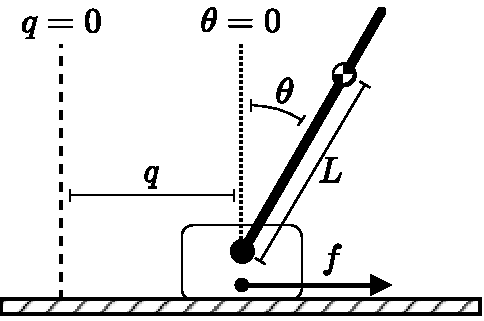
\includegraphics[width=\textwidth]{assets/pic}
        \caption{aaaaa}
        \label{fig:pic}
    \end{subfigure}
    \hfill
    \begin{subfigure}[b]{0.48\textwidth}
        \centering
        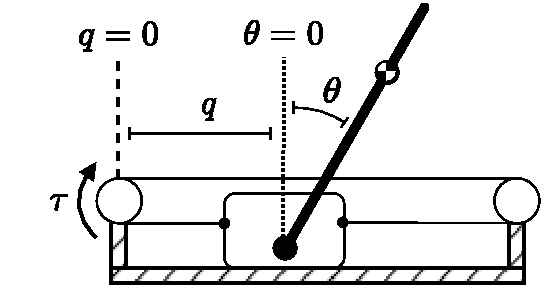
\includegraphics[width=\textwidth]{assets/pic-real}
        \caption{bbbbb}
        \label{fig:pic-real}
    \end{subfigure}
    \caption{Schema del sistema.} %todo
\end{figure}
